\documentclass{mcmthesis}
\mcmsetup{CTeX = false,    % 使用 CTeX 套装时,设置为 true
	tcn = {2504496}, problem = \textcolor{red}{A},
	sheet = true, titleinsheet = true, keywordsinsheet = true,
	titlepage = false, abstract = false}

\usepackage{newtxtext}     % \usepackage{palatino}
\usepackage[style=ieee,backend=biber]{biblatex}
\addbibresource{reference.bib}

\usepackage{tocloft}
\setlength{\cftbeforesecskip}{6pt}
\renewcommand{\contentsname}{\hspace*{\fill}\Large\bfseries Contents \hspace*{\fill}}

\usepackage{enumitem}

\usepackage{algorithm}
\usepackage{algpseudocode}
\usepackage[table,xcdraw]{xcolor}
\usepackage{booktabs}

\usepackage[table]{xcolor} % 只加载一次
\usepackage{array, booktabs, tabularx}
\usepackage{fancyhdr}
\setlength{\headheight}{13.6pt} % 解决fancyhdr警告
\newcolumntype{Y}{>{\raggedright\arraybackslash}X} % 自适应列


% 定义轻微的蓝色和灰色
\definecolor{lightgray}{rgb}{0.9, 0.9, 0.9}
\definecolor{lightblue}{rgb}{0.757, 0.989, 0.902}

\setlength{\arrayrulewidth}{0.5mm} % 横线加粗
\setlength{\tabcolsep}{12pt} % 设置表格列间距



\title{Enjoy a Cozy and Green Bath}
% \author{\small \href{http://www.latexstudio.net/}
	%   {\includegraphics[width=7cm]{mcmthesis-logo}}}
\date{\today}

\begin{document}
	
	%%%%%%%%%%%%%%%%%%%%%%%%%%%%%%%%%%%%%%%%
	%%%%%%%%%%%%%%%%% 摘要 %%%%%%%%%%%%%%%%%
	%%%%%%%%%%%%%%%%%%%%%%%%%%%%%%%%%%%%%%%%
	\begin{abstract}
		
		abstract...
		
		\begin{keywords}
			Keyword one, Keyword two, Keyword three
		\end{keywords}
		
	\end{abstract}
	
	
	\maketitle
	\tableofcontents        % 若不想要目录, 注释掉该句
	\thispagestyle{empty}
	\newpage
	
	
	
	
	
	%%%%%%%%%%%%%%%%%%%%%%%%%%%%%%%%%%%%%%%%
	%%%%%%%%%%%%%%%%% 引言 %%%%%%%%%%%%%%%%%
	%%%%%%%%%%%%%%%%%%%%%%%%%%%%%%%%%%%%%%%%
	
	
	\section{Introduction}
	
	\subsection{Background}
	The medal table of the 2024 Paris Olympics shows that the United States and China each won 40 gold medals and tied for the top spot, but the United States led with a total of 126 medals. The host country France ranked fifth in gold medals (16) and fourth in total medals (64). Dominica, Saint Lucia and other countries won their first Olympic medals, while 60 countries still have not broken through for any medals.
%	\begin{figure}[htbp]
%		\centering
%		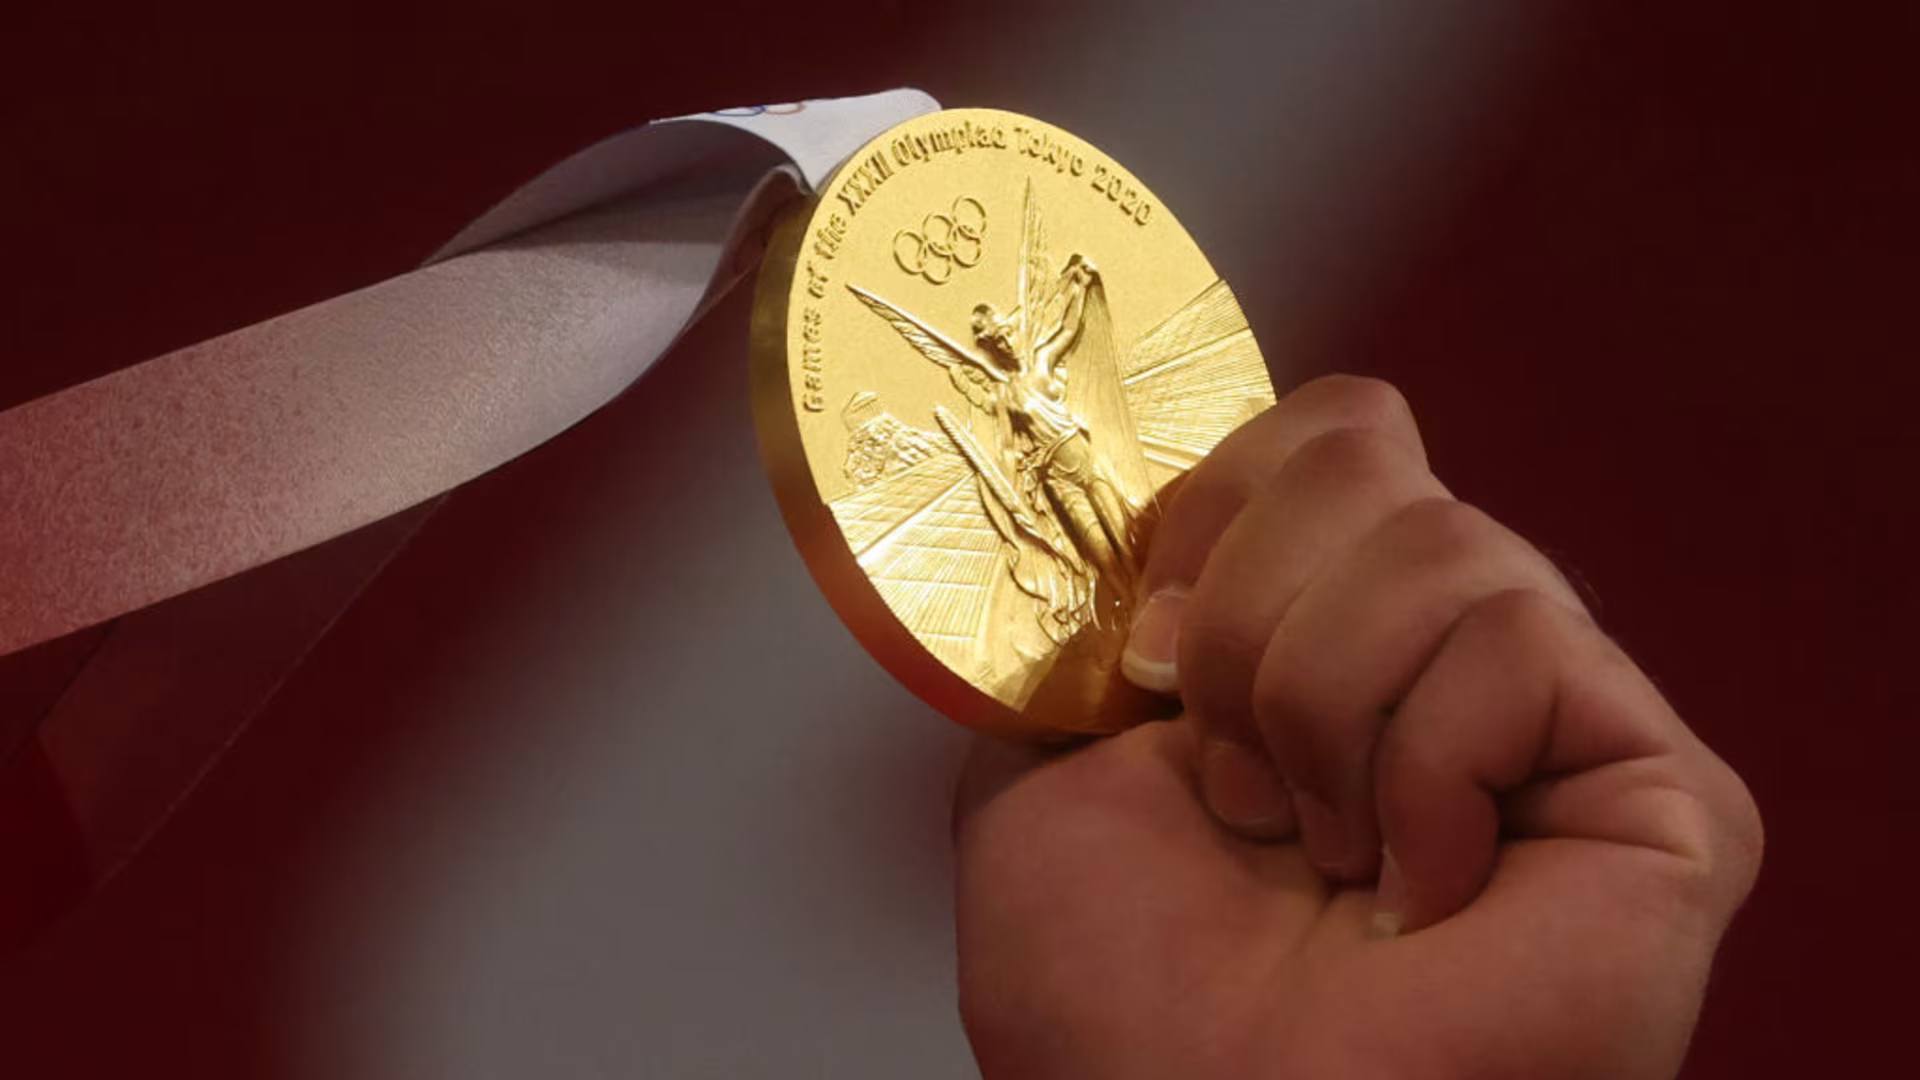
\includegraphics[width=0.7\linewidth]{fig/background}
%		\caption{The medals of the 2024 Paris Olympics}
%	\end{figure}
	
	\subsection{Restatement and Analysis of the Problem}
	Based on the provided historical data-set of the Olympic Games from 1896 to 2024, we are employed to analyze and answer the following questions:
	\begin{enumerate}
		\item 
		Develop a \textbf{prediction model} to forecast the number of medals each country will win in 2028, and identify countries that may progress or regress. 
		\item 
		Provide \textbf{prediction intervals} and estimates of \textbf{uncertainty} and metrics to measure the model's performance.
		\item 
		Estimate the number of countries that will win their \textbf{first medal} and the probability of this happening.
		\item 
		Analyze the \textbf{relationship} between specific Olympic events (in terms of quantity and type) and the number of medals, explore which events are more important, and the impact of the host country's event selection strategy on the outcome.
		\item 
		Verify whether the \textbf{mobility of coaches} significantly enhances a country's performance in specific sports (such as Lang Ping and Bela Karolyi).
		\item 
		Quantify the contribution of\textbf{ coaching effectiveness} to the number of medals, and recommend key sports for investment and expected returns for the three countries.
		\item 
		Extract the less-attended-to patterns from the model and provide strategic \textbf{suggestions} for the Olympic Committee.
	\end{enumerate}
	
	For Task 1, we selected seven indicators and established an LSTM-based medal quantity prediction model, and provided interval predictions using Bayesian estimation. As for countries that have never won medals, we built an SVM-based "first medal breakthrough" prediction model based on the new events, the number of athletes, and historical participation trends.
	
	
	%对于Task1,我们选取7个指标,建立了基于LSTM的奖牌数量预测模型,并使用贝叶斯估计给出了区间预测,而对于从未获奖的国家,我们根据新增的event、运动员数量、历史参与趋势,建立了基于SVM的“首奖突破”预测模型。
	%对于Task2,我们分析了“伟大教练”效应的影响。
	
	
	
	
	
	
	
	
	
	\subsection{Overview of Our Work}
	
	%\begin{itemize}
	%	\item {\bf 111}. ...
	%	\item {\bf 222}. ...
	%	
	%	\begin{itemize}
		%		\item[1)] ... 
		%		\item[2)] ...
		%		\item[3)] ...
		%		\item[4)] ...
		%	\end{itemize}
	%	
	%\end{itemize}
	
	
	
	
	
	
	
	
	%%%%%%%%%%%%%%%%%%%%%%%%%%%%%%%%%%%%%%%%
	%%%%%%%%%%%%%%%%% 模型假设 %%%%%%%%%%%%%%%%%
	%%%%%%%%%%%%%%%%%%%%%%%%%%%%%%%%%%%%%%%%
	\section{Assumptions and Justification}
	
	To simplify the problem and make it convenient for us to simulate real-life 
	conditions, we make the following basic assumptions, each of which is properly 
	justified.
	
	\begin{itemize}
		\item {\bf 1}. ...
		\item {\bf 2}. ...	
	\end{itemize}
	
	
	
	
	
	
	
	
	
	
	%%%%%%%%%%%%%%%%%%%%%%%%%%%%%%%%%%%%%%%%
	%%%%%%%%%%%%%%%%% 符号说明 %%%%%%%%%%%%%%%%%
	%%%%%%%%%%%%%%%%%%%%%%%%%%%%%%%%%%%%%%%%
	\section{List of Notations}
	\begin{center}
		\begin{tabular}{ll}
			\toprule
			{\bf Symbols} & {\bf Description}  \\
			\midrule 
			$A_{C},A_{S}$ & Set of country, all sports in Olympic.\\
			$A_{T}$ & $\{1,\dots,30\}$, representing the ordinal number of year Olympic held. \\
			$A_{H}(t)$ & Set of host country in year $t$. \\
			$MG_{t,i,j,k}$ & Number of gold medals country $i$ won in sport $j$ at event $k$ in year t. \\
			$MS_{t,i,j,k}$ & Number of silver medals country $i$ won in sport $j$ at event $k$ in year t. \\
			$MB_{t,i,j,k}$ & Number of bronze medals country $i$ won in sport $j$ at event $k$ in year t. \\
			$MT_{t,i}$ & Number of total medals country $i$ won in year $t$. \\
			$N_{athletes}(t,i)$ & Total number of athletes from country $i$ in year $t$. \\
			$N_{award}(t,i)$ & Number of athletes who won medals from country $i$ in year $t$. \\
			$H(t,i)$ & Host effect. \\
			$G_{\text{growth}}(t,i)$ & Growth rate of the number of athletes from country $i$ in year $t$.\\
			$P_{Medal}(t,i)$ & Probability of country $i$ winning a medal in year $t$.\\
			$P_{Gold}(t,i)$ & Probability of country $i$ winning a gold medal in year $t$.\\
			\bottomrule
		\end{tabular}
	\end{center}
	
	\noindent Note: The Summer Olympics have been held for a total of 32 sessions.
	
	
	
	
	
	
	
	
	
	%%%%%%%%%%%%%%%%%%%%%%%%%%%%%%%%%%%%%%%%
	%%%%%%%%%%%%%%%%% 数据预处理 %%%%%%%%%%%%%%%%%
	%%%%%%%%%%%%%%%%%%%%%%%%%%%%%%%%%%%%%%%%
	\section{Data Pre-processing}
	
	\subsection{Outlier and Missing Value Handling}
	As the \textbf{1906 Intercalated Games} lacked the medal data of various countries and the competition results were not recognized by the International Olympic Committee, the data of 1906 is not taken into account.
	
	In adition, \textbf{Skating} and \textbf{Ice Hockey} have been included in the Winter Olympics since 1920, so these two events are not within the scope of consideration. Otherwise, the "$\cdot$" is replaced by the number $0$. 
	
	It was noticed that \textbf{Jeu de Paume} and \textbf{Roque} sports in the {\bf summerOly\_programs.csv} do not have Codes. Upon researching information from {\color{blue}\url{https://en.wikipedia.org/wiki/Jeu_de_paume}} and {\color{blue}\url{https://en.wikipedia.org/wiki/Roque}}, it was found that only a few people are still engaged in these two sports, which have even not been held for 26 consecutive years in the Summer Olympics. Therefore, these two sports have been excluded.
	
	%\section{Descriptive statistical analysis}
	
	苏联、俄罗斯
	
	
	
	
	
\begin{itemize}[leftmargin=0.15in, labelsep=0.1in, itemsep=1pt, parsep=0pt]
	\item aAAAAAAAA
	\item BBBBBBBBBB
\end{itemize}


	
	
	
	
	
	
	%%%%%%%%%%%%%%%%%%%%%%%%%%%%%%%%%%%%%%%%
	%%%%%%%%%%%%%%%%% Task 1 %%%%%%%%%%%%%%%%%
	%%%%%%%%%%%%%%%%%%%%%%%%%%%%%%%%%%%%%%%%
	\section{Task 1: How Many Medal Counts in 2028? }
	
	\subsection{Significance Analysis of Host Effect}
	
	Host Effect refers to the phenomenon where a host country tends to perform better in large-scale international events (such as the Olympic Games or the World Cup) due to the advantages associated with competing on home soil. This often manifests in a significant increase in the host country's medal count, competition results, and overall performance.
	
	%为了验证东道主效应的显著性,我们采用了成对样本t检验。首先,我们选取每年的东道主的奖牌数$MT_{ti}$作为第一个样本,其次,为了消除奖牌数量的整体增长趋势的影响,选取东道主国家在前后两届奥运会中获得的奖牌数的平均值
	
	To assess the significance of the host effect, we employed a paired samples  \textbf{t-Test}. First, we selected the medal count of the host country for each year, denoted as $MT_{t}$, as the first sample. To eliminate the influence of overall growth trends in medal counts, we used the average medal count from the two preceding Olympic Games as the second sample, as shown in equation (\ref{eq:H_t-test_MT_bar}),
	\begin{equation}
		MT^H_{t}=\frac{ MT_{t-1} + MT_{t+1} }{2}
		\label{eq:H_t-test_MT_bar}
	\end{equation}
	where $t=2,3,\cdots,29$, $i\in A_{C}$. 
	
	The data set $\{MT_{t},MT^s_{t}\}$ then forms a paired sample with a size of 30. 
	
	Define $d_t= MT_{t} - MT^s_{t}$, and assume that
	\begin{equation*}
		H_0: \mu_d=0, \quad vs \quad H_1:  \mu_d \ne 0.
	\end{equation*}
	
	Select the t-test statistic as
	\begin{equation}
		T=\frac{ \bar{d} }{ s_d\slash \sqrt{28} } \sim (27)
	\end{equation}
	where $\bar{d}=\frac{1}{28} \sum_{t=2}^{29} d_t$ is the mean of paired samples, 
	and $ s_d = \frac{1}{27} \sum_{t=2}^{29}\big( d_t - \bar{d} \big)^2 $ is the sample variance of the differences of paired data, 
	
	For a given significance level $\alpha$, the rejection domain for the hypothesis test is
	\begin{equation}
		W_\alpha = \big\{ |T| \ge t_{1-\frac{\alpha}{2}}(29) \big\}
	\end{equation}
	
	By following the described procedure, the results of the t-test were obtained and are summarized in Table \ref{table:H_t-test_result}.
	
	结果待写
	
	
	
	\subsection{Analysis of Key Indices}
	\subsubsection{Host effect}
	
	Define Logical Variable $H_{t,i}$ as equation (\ref{eq:H}),
	\begin{equation}
		H(t,i)=
		\begin{cases}
			1, \quad \text{Country } i \text{ is host in year } t, \\
			0, \quad \text{others}.
		\end{cases}
		\label{eq:H}
	\end{equation}
	where $t\in A_{T}$, $i\in A_{C}$.
	
	
	
	\subsubsection{Event held}
	The event vector \( V(t) \) is defined as:
	
	\[
	V(t) = \big( v_1(t), v_2(t), \dots, v_M(t) \big)^T,
	\]
	where: \( v_i(t) = 1 \) if event \( i \) is held in year \( t \),
	\( v_i(t) = 0 \) if event \( i \) is not held in year \( t \). Here, \( M \) represents the total number of distinct Olympic events considered up to year \( t \) ($t=1,2,\cdots,30$) and the elements of \( V(t) \) are binary values indicating the participation of each event in year \( t \).
	
	
	
	\subsubsection{Definition of Dominant Event}
	
	Let \( I_j(t) \) represent the dominance of event \( j \) in year \( t \), where the dominance is calculated based on the medal count over the past three years and the total number of medals in year \( t \).
	
	\[
	I_j(t) = \frac{\sum_{q=t-3}^{t-1} MT_{q,i,k,j}}{\sum_{q=t-3}^{t-1} V_j(q) \cdot MT_{q,i,j,k}} 
	\]
	
	Next, define \( I(t) = \big( I_1(t), I_2(t), \dots, I_M(t) \big)^T \) as the dominance vector. 
	
	To get the modified dominance vector \( I'(t) \), we set the components corresponding to the three largest values of \( I(t) \) to 1, and all other components to 0:
	
	\[
	\hat{I}(t) = 
	\begin{cases} 
		1 & \text{if } j \in \text{Top3}(I(t)) \\
		0 & \text{otherwise}
	\end{cases}
	\]
	
	\[\hat{I}(t) = \mathbf{1}_{\{ j \in \text{Top3}(I(t)) \}},\]
	where \( \text{Top3}(I(t)) \) refers to the indices corresponding to the three largest values in the vector \( I(t) \), and \( \mathbf{1} \) is the indicator function.
	
	
	\subsubsection{Strong Events}
	
	Let \( \hat{I}(t) \) and \( V(t) \) be the dominance vector and the event vector for year \( t \), respectively. The number of strongpoints \( S(t) \) can be defined as:
	\[
	S(t) = \sum_{i=1}^{M} \mathbf{1}\{ \hat{I}_i(t) = 1 \text{ and } v_i(t) = 1 \},
	\]
	where \( \mathbf{1}\{ \cdot \} \) is the indicator function, which is 1 if the condition inside the curly brackets is true and 0 otherwise. 
	In this context, \( \hat{I}_i(t) = 1 \) means that event \( i \) has a dominant position in year \( t \), and \( v_i(t) = 1 \) indicates that event \( i \) is held in year \( t \).
	
	
	\subsubsection{Percentage of winners}
	\[R(t,i) = \frac{N_{\text{award}}(t,i)}{N_{\text{athletes}}(t,i)}\]
	
	\subsubsection{Medal Distribution Concentration}
	\[
	\text{HHI}(t,i) = \sum_{j=1}^{M} \left( \frac{MT_{t,i,j}(t)}{MT_{t,i}(t)} \right)^2
	\]
	where the closer the \textbf{HHI}(Herfindahl-Hirschmann Index)\cite{HHI2016} is to 1, the more concentrated the distribution of medals is in a small number of sports, and the closer it is to 0, the more widely distributed the medals are.
	
	\subsubsection{historical performance}
	
	\[
	\widetilde{MT}(t,i) = \frac{1}{3} \sum_{q=t-3}^{t-1} MT_{q,i}
	\]
	
	
	\subsection{Prediction of Medal Count for Medal-Winning Countries Using LSTM}
	x x\cite{Gal2015DropoutAA}
%	\begin{figure}[H]
%		\centering
%		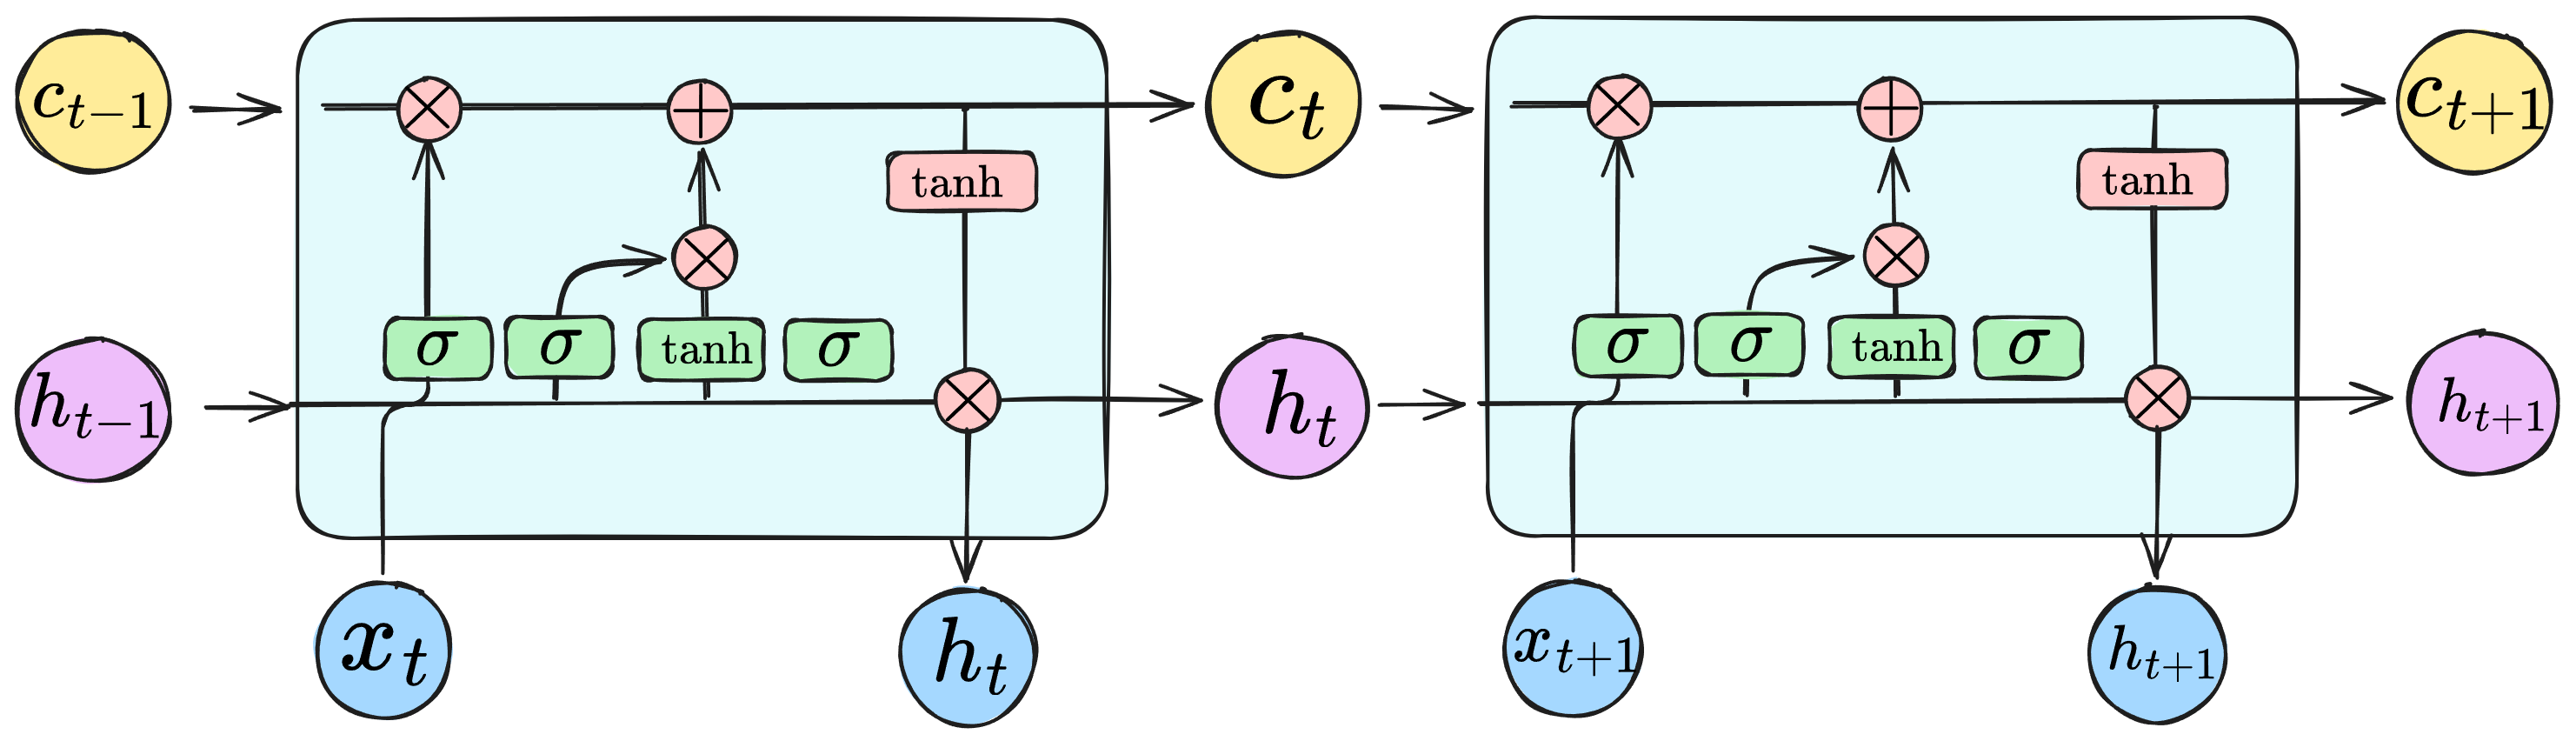
\includegraphics[width=1\linewidth]{fig/LSTM2.png}
%		\caption{Flow of LSTM based on Monte Carlo Dropout}
%		\label{fig:LSTM}
%	\end{figure}
	\begin{algorithm}
		\caption{LSTM Medal Prediction with Uncertainty Quantification}
		\begin{algorithmic}[1]
			\State \textbf{Input:} Historical sequence \( X = [H(t,i), S(t), R(t,i), HHI(t,i), \widetilde{MT}(t,i), N_{\text{athletes}}(t,i)] \)
			\State \textbf{Initialize:} Parameters \( \theta = \{W_f, W_i, W_o, W_c, b_f, b_i, b_o, b_c\} \)
			\State Initialize hidden state \( h_0 \gets \mathbf{0} \), cell state \( c_0 \gets \mathbf{0} \)
			\State Set dropout rate \( p = 0.4 \), Monte Carlo samples \( M = 100 \)
			
			\For{each \( t = 1 \) to \( T \)}
			\State Compute forget gate \( f_t = \sigma(W_f[h_{t-1}, x_t] + b_f) \)
			\State Compute input gate \( i_t = \sigma(W_i[h_{t-1}, x_t] + b_i) \)
			\State Compute candidate state \( \tilde{c}_t = \tanh(W_c[h_{t-1}, x_t] + b_c) \)
			\State Update cell state \( c_t = f_t \odot c_{t-1} + i_t \odot \tilde{c}_t \)
			\State Compute output gate \( o_t = \sigma(W_o[h_{t-1}, x_t] + b_o) \)
			\State Update hidden state \( h_t = o_t \odot \tanh(c_t) \)
			\EndFor
			
			\For{each \( m = 1 \) to \( M \)}
			\State Enable dropout masks \( \xi^{(m)} \sim \text{Bernoulli}(p) \)
			\State Compute prediction \( \hat{y}^{(m)} \gets \text{LSTM}(X; \theta, \xi^{(m)}) \)
			\EndFor
			
			\State Compute prediction mean \( \mu_y = \frac{1}{M}\sum_{m=1}^M \hat{y}^{(m)} \)
			\State Compute standard deviation \( \sigma_y = \sqrt{\frac{1}{M}\sum_{m=1}^M (\hat{y}^{(m)} - \mu_y)^2} \)
			\State Compute 95\% confidence interval \( \text{CI}_{95\%} = [\mu_y - 1.96\sigma_y, \mu_y + 1.96\sigma_y] \)
			
			\State Compute loss \( \mathcal{L} = \frac{1}{N}\sum_{i=1}^N (\hat{y}_i - y_i^{\text{true}})^2 \)
			\State Backpropagate gradients \( \nabla_\theta \mathcal{L} \) via BPTT
			\State Update parameters \( \theta \gets \theta - \eta \nabla_\theta \mathcal{L} \) \(\quad \text{(where \( \eta \) is the learning rate)}\)
			
			\State \textbf{Return:} \( \mu_y, \text{CI}_{95\%} \)
		\end{algorithmic}
	\end{algorithm}
	
	
	% 修正后的表格
	\begin{table}[H]
		\centering
		\caption{LSTM Model Parameters Specification}
		\label{tab:lstm_params}
		\renewcommand{\arraystretch}{1}
		\small
		\begin{tabularx}{\textwidth}{lYcc}
			\toprule
			\rowcolor{lightblue!20}
			\textbf{Parameter} & \textbf{Description} & \textbf{Dimensions} & \textbf{Activation} \\
			\midrule
			
			\rowcolor{gray!10}
			$W_f$ & Forget gate weight matrix & $[h_{t-1}+x_t]$ & Sigmoid \\
			$W_i$ & Input gate weight matrix & $[h_{t-1}+x_t]$ & Sigmoid \\
			\rowcolor{gray!10}
			$W_o$ & Output gate weight matrix & $[h_{t-1}+x_t]$ & Sigmoid \\
			$W_c$ & Candidate cell state weights & $[h_{t-1}+x_t]$ & Tanh \\
			\rowcolor{gray!10}
			$b_f, b_i, b_o, b_c$ & Bias vectors & $[1]$ & -- \\
			$h_t$ & Hidden state output & $[N]$ & -- \\
			\rowcolor{gray!10}
			$c_t$ & Cell state output & $[N]$ & -- \\
			$y_{\text{pred}}$ & Predicted medal count & Scalar & Linear \\
			\rowcolor{gray!10}
			$y_{\text{true}}$ & Actual medal count & Scalar & -- \\
			\textbf{Init} & Xavier initialization & $[N]$ & -- \\
			\bottomrule
		\end{tabularx}
	\end{table}
	
	
	
	
	
	
	\subsection{Uncertainty estimation Monte Carlo Dropout}
	
	%在体育赛事中,往往会有例如受伤等突发事件,充满了不确定性,Monte Carlo Dropout 可以为模型提供不确定性估计。
	
	In sports events, there are often unexpected incidents such as injuries, which are full of uncertainties for Olympics. The Monte Carlo Dropout (MC Dropout) can quantify uncertainty of the model \cite{gal2016dropout}.
	
	The uncertainty is estimated by generating the distribution of predicted values through multiple random activation of the Dropout layer during the inference stage. By conducting multiple forward passes, the variance of the model's output is used to measure the confidence of the prediction.
%	
%	\begin{figure}
%		\centering
%		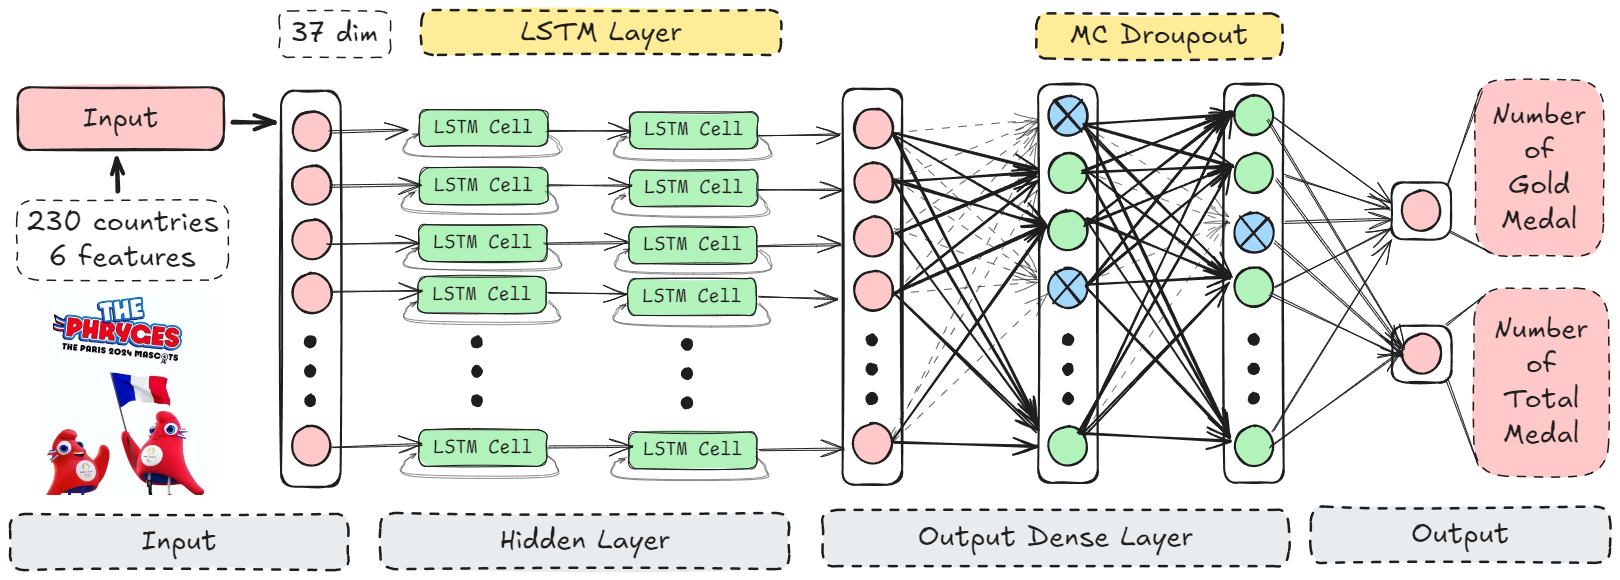
\includegraphics[width=1\linewidth]{fig/LSTM-MCD.png}
%		\caption{Flow of LSTM based on Monte Carlo Dropout}
%		\label{fig:lstm-mcd}
%	\end{figure}
	
	
	Assume $f(x;\theta)$ is the prediction model we build, $x$ is its input and $\theta$ is parameters. In the training stage, Dropout operates with a probability $p$
	randomly dropping neurons is equivalent to sampling from the posterior distribution $P(\theta|D)$ ($D$ are training data) of the parameters. In the inference stage, perform forward propagations $32$ times before each time, generating a mask $\{f(x;\theta,m_t)\}_{t=1}^{30}$ each time. Then, the calculation of the predicted mean and variance is as follows:
	\begin{align*}
		\hat{y}&=\frac{1}{32} \sum_{t=1}^{32} f(x;\theta,m_t) \\
		Var(y) &=\frac{1}{32} \sum_{t=1}^{32} \big( f((x;\theta,m_t)) - \hat{y} \big)^2
	\end{align*}
	where $Var(y)$ reflects the predictive uncertainty of the model for the input $x$.
	
	The results is shown as Figure \ref{}.
	
	
	
	
	
	
	\section{Task 2}
	
	
	\subsection{Problem Overview}
	The objective of this model is to predict whether countries that have never won a medal in the past (i.e., "first-time winning countries") will be able to win a medal in future Olympic Games. For these countries, traditional medal prediction models (which usually rely on historical medal data) may not effectively predict their future performance. Therefore, we need to consider other potential factors, such as the host country effect, athlete participation growth, and the addition of new events.
	
	
	\subsection{Index Analysis}
	
	
	\subsubsection{Target variable}
	\[
	y(t,i) = 
	\begin{cases} 
		1 & \text{if country } i \text{ wins a medal in year } t \\ 
		0 & \text{if country } i \text{ does not win a medal in year } t 
	\end{cases}
	\]
	\subsubsection{Athlete growth rate}
	The growth rate of athletes from country $i$ in year $t$, calculated by the following formula:
	\[
	G_{\text{growth}}(t,i) = \frac{N_{\text{participate}}(t,i) - N_{\text{participate}}(t-1,i)}{N_{\text{participate}}(t-1,i)}
	\]
	where $N_{\text{participate}}(t,i)$ is the number of athletes from country $i$ in year $t$.
	
	
	\subsubsection{Participation in new events compared to previous years} 
	\begin{algorithm}
		\caption{Participation in new events compared to previous years}
		\begin{algorithmic}[1]
			\State \textbf{Input:} Year \( t \), Country \( i \), Matrices \( N_{\text{new}} \), \( P_{\text{new}} \)
			\For {each \( k \in \{t-2, t-1, t\} \)}
			\If {$N_{\text{new}}[k][i] > 0$ \textbf{and} $P_{\text{new}}[t][i] > 0$}
			\State \textbf{Return} $\min(N_{\text{new}}[t][i], P_{\text{new}}[t][i])$
			\EndIf
			\EndFor
			\State \textbf{Return} 0
		\end{algorithmic}
	\end{algorithm}
	
	where \( N_{\text{new}}(t,i) \) represents the number of new events that country \( i \) participated in during year \( t \), and \( P_{\text{new}}(t,i) \) indicates the quantity of new events in which country \(i\) participated during year. We define \( \tilde{N}_{\text{new}} = \min(N_{\text{new}}[t][i], P_{\text{new}}[t][i]) \).
	
	
	
	
	
	
	\subsection{Prediction model:}  
	We use a Random Forest (RF) classifier to predict whether first-time winning countries will win medals. The model’s input is the feature vector of the country \( X(t,i) \):
	
	\[
	X(t,i) = [G_{\text{growth}}(t,i), H(t,i), \tilde{N}_{\text{new}}(t,i)]
	\]
	
	The RF classifier consists of multiple decision trees, where each tree makes a prediction, and the final prediction is determined by majority voting from all the trees:
	
	\[
	P(\text{Medal}(t,i)) = \frac{1}{T} \sum_{t=1}^{T} f_t(X(t,i), \theta_t)
	\]
	
	where \( T \) is the number of trees in the forest, \( f_t(\cdot) \) is the decision function of the \( t \)-th tree, and \( \theta_t \) is the parameter learned during training for the \( t \)-th tree.
	
	\textbf{Prediction of first-time medal probability:}  
	If country \( i \) has never won a medal (i.e., no historical medals), we use the RF classifier to calculate the probability of winning a medal. If the probability exceeds a certain threshold, we predict that the country may win a medal in the future, especially a first-time medal:
	
	\[
	P_{Medal}(t,i) > \text{Threshold}
	\]
	
	where the threshold is determined based on the results of model evaluation.
	\begin{algorithm}
		\caption{Prediction with Random Forest for First-Time Medal}
		\begin{algorithmic}[1]
			\State \textbf{Input:} Year \( t \), Country \( i \), Matrices \( \tilde{N}_{\text{new}} \), \( P_{\text{new}} \), Feature vector \( X(t,i) \), RF with \( T \) trees.
			\State \textbf{Output:} First-time medal prediction probability \( P_{\text{first medal}}(t,i) \)
			
			\State Calculate feature vector \( X(t,i) = [G_{\text{growth}}(t,i), H(t,i), N_{\text{new}}(t,i)] \)
			
			\State Initialize prediction sum: \( P_{\text{sum}} = 0 \)
			
			\For {each tree \( t \in \{1, \dots, T\} \)}
			\State Get prediction from tree \( t \): \( p_t = f_t(X(t,i), \theta_t) \)
			\State Update prediction sum: \( P_{\text{sum}} = P_{\text{sum}} + p_t \)
			\EndFor
			
			\State Calculate average prediction: \( P_{Medal}(t,i)  = \frac{P_{\text{sum}}}{T} \)
			
			\If { \( P_{Medal}(t,i) > \text{Threshold} \) }
			\State \textbf{Return} 1 \text{ (Predicted to win first medal)}
			\Else
			\State \textbf{Return} 0 \text{ (Predicted not to win first medal)}
			\EndIf
		\end{algorithmic}
	\end{algorithm}
	
	
	
	
	
	
	
	
	
	
	
	
	
	
	
	
	
	
	
	
	
	\section{Task 3: xxx}
	
	
\section{Task 4: Effect of Great Coach}
	

	
\subsection{Test of Parallel Trend }
%我们可以从图4中看出,从1900年-1984年,美国体操队的奖牌数与xx国相似,为了证实这一猜想,我们对他们的奖牌数进行平行检验,

We can see that the number of medals won by the US gymnastics team from 1896 to 1984 and 1984-2016 years in Figure \ref{fig: parallel_trend}. To verify this conjecture, we conducted a parallel test on their medal counts.


\subsection{Test of Great Coach Effect based on DiD}

To seek evidence of the existence of the great coach effect, we employ the Difference-in-Differences (DiD) model to examine its impact.

The DiD model is a statistical method used to assess the causal effect of an intervention on an outcome variable. It estimates the intervention effect by comparing the performance differences between the experimental group and the control group before and after the intervention. The model equation is 
\begin{equation}
Y_{i,t}=\alpha+\delta_t+\gamma \cdot Treat_i \cdot Post_t + \varepsilon_{i,t},
\end{equation}
where \( Y_{i,t} \) represents team \( i \)'s performance at time \( t \) (e.g., medal count). The model includes a constant term \(\alpha\), time fixed effects \(\delta_t\) for common influences (e.g., 1980s gymnastics improvements), and an interaction term \( Treat_i \cdot Post_t \) to capture \textbf{Béla Károlyi}'s impact as coach on the U.S. team. The coefficient \(\gamma\) measures the "great coach effect," and \(\varepsilon_{i,t}\) is the error term.

By using $Least$ $Squares$ $Method$ in $Python$, we obtained the estimated value of the regression coefficient $\hat{\gamma}=4.1572$. To test the significance of $\gamma$, assume that
\begin{equation*}
H_0: \gamma=0 \quad vs \quad H_1: \gamma>0
\end{equation*}

Select the test statistic:
\begin{equation}
T=\frac{ \hat{\gamma} }{ \text{SE}(\hat{\gamma}) } \sim t(30-4)
\end{equation}
where $\text{SE}(\hat{\gamma}) = \sqrt{ \frac{1}{N} \sum_{i=1}^{N} \hat{\varepsilon}_i^2 }$, $\hat{\varepsilon}=\hat{Y}_{i,t}-Y_{i,t}$. For a given significance level $\alpha$, the rejection domain for the hypothesis test is
\begin{equation}
	W_\alpha = \big\{ |T| \ge t_{1-\frac{\alpha}{2}}(30-4) \big\}
\end{equation}

The test results of regression coefficients were obtained and are summarized in Table \ref{table:great-coach-effect_t-test}. The sample falls within the rejection region $W_{0.975}$, so it can be concluded that the regression coefficient $\gamma$ is significant, e.i. the impact of great coach Béla Károlyi for the USA gymnastics team is significant. On average, a great coach can increase the number of medals by 4 for the US gymnastics.
\begin{table}[H]
	\centering
	\caption{Transposed Presentation of t-Test Results}
	\label{table:great-coach-effect_t-test}
	\begin{tabular}{lcccc}
		\toprule
		\rowcolor{red!10}
		& \textbf{t-statistic} & \textbf{p-value} & \textbf{Critical value (α=0.05)} & \textbf{Test conclusion} \\
		\midrule
		\rowcolor{white} % 纯白色
		\textbf{Value} & 3.045 & 0.008 & 2.052 & Reject null hypothesis \\
		\bottomrule
	\end{tabular}
\end{table}




\subsection{Selection of Investment Sports}

%一般国力雄厚的国家能够花费金钱聘请优秀教练,所以我们最好选择有一定实力但不是非常顶尖的国家。考虑到一代运动员的职业生涯一般为4届运动会,故统计2012、2016、2020、2024这四届奥林匹克运动会的奖牌总数总和,并排序,如图所示

Generally, countries with strong national power can afford to hire excellent coaches, so we'd better choose countries that have certain strength but are not the very top ones. Considering that an athlete's career usually lasts for 4 Olympic Games, the total number of medals won in the 2012, 2016, 2020 and 2024 Olympic Games was calculated and ranked, seeing Figure \ref{fig:medal_count_by_noc}.

\begin{figure}[H]
	\centering
	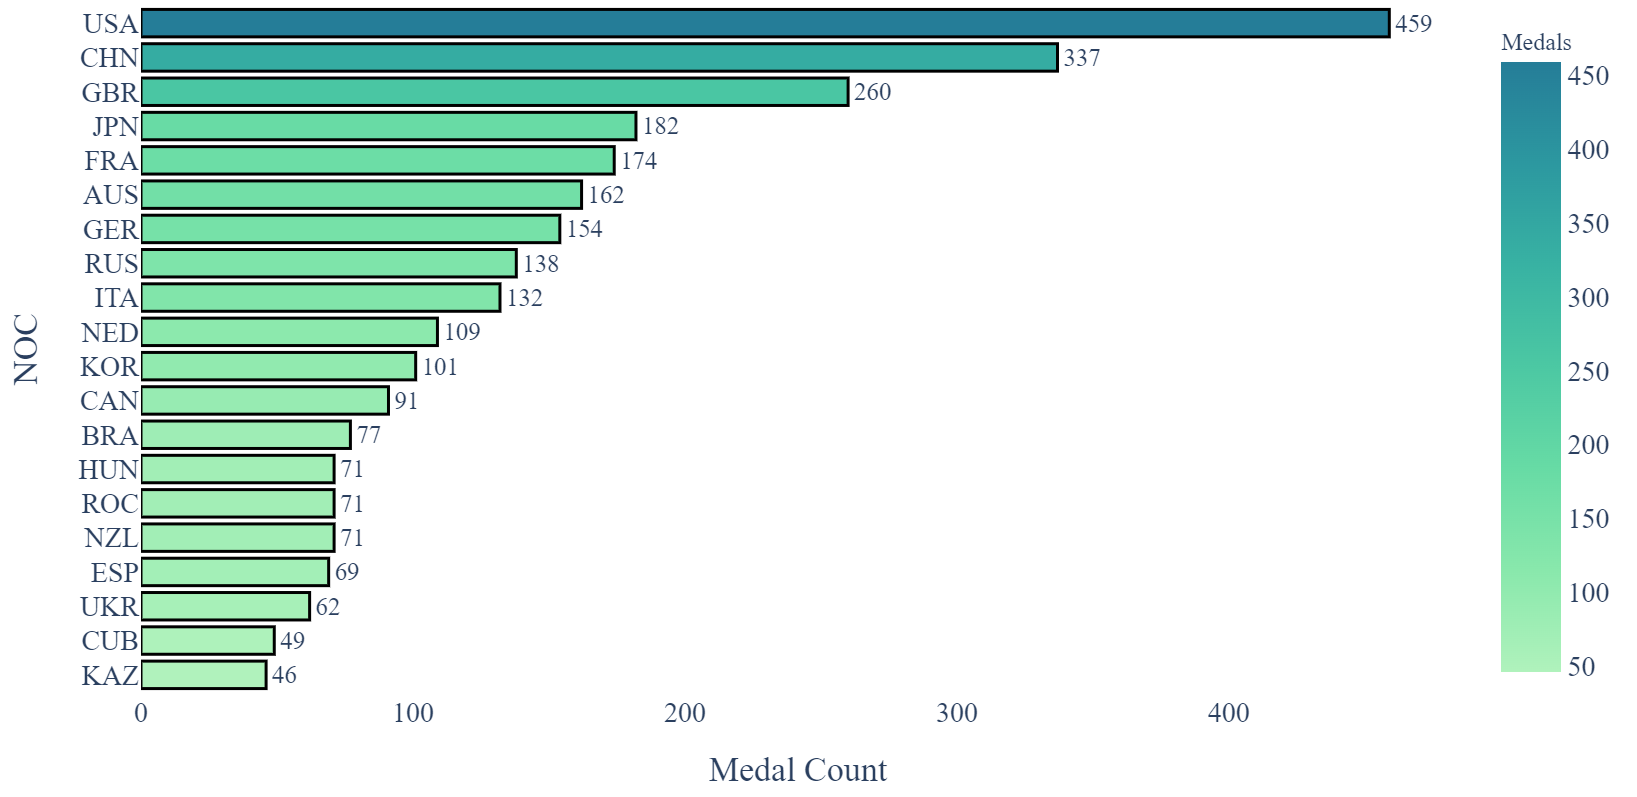
\includegraphics[width=1\linewidth]{fig/Medal_Count_by_NOC.png}
	\caption{Sort of Various Conutries by Total Medal Count}
	\label{fig:medal_count_by_noc}
\end{figure}

%根据图2,美国、中国、英国排在TOP3,而日本、法国、澳大利亚排在第4-6名,后者都属于有较为雄厚的国力且有提升潜力的国家,故而选择日本、法国、澳大利亚这三个国家进行分析。
%我们选择对日本、法国、澳大利亚这三个国家提出投资建议

Based on Figure \ref{fig:medal_count_by_noc}, the United States, China, and the United Kingdom occupy the TOP 3 positions in terms of medal counts. Japan, France, and Australia rank 4-6, respectively. Given that these latter three countries possess substantial national resources and demonstrate significant potential for improvement, We choose to offer investment suggestions for Japan, France and Australia.

%最需要考虑的项目最好是"汇报/投入"最大的项目,故对每个项目,因为团体项目人数多但是奖牌少,即选择奖牌数回报率更高的国家,奖牌数回报率被定义为式3

%故对每个项目,因为团体项目人数多但是奖牌少

The item that requires the most consideration is preferably the one with the greatest "return on input", namely, to select the country with a higher medal return rate. The \textbf{Medal Return Rate} is defined as Eq(\ref{eq:MRR}).
\begin{equation}
MRR_{i,j}=1-\text{Normal}
\Bigg( 
\frac{ \sum_{t=27}^{30} \sum_{k\in \tilde{A}_{E}(j)} MT_{t,i,j} }{ \sum_{t=27}^{30} \sum_{j\in \tilde{A}_{S}} N_{athletes}(t,i,j) }
\Bigg)
\label{eq:MRR}
\end{equation}
where $\tilde{A}_{E}(j)$ denotes individual event of sport $j$, and $\text{Normal}(x)=x/(\max{x} - \min{x})$. 

The larger the $MRR$ is, the more people are involved in the single-person sport but the fewer awards are won, indicating a greater potential for medal count improvement. After calculation, $MRR_{i,j}$ are shown in Table \ref{table:MRR}.

%MRR越大,表示这个单人项目人数多但是获奖少,有更高的奖牌数提升潜力,经过计算,如表3所示






	\section{Task 5}
	
	\section{Sensitivity Analysis}
	
	\section{Strength and Weakness}
	\subsection{Strength}
	\subsection{Weakness}
	
	\section{Further Discussion}
	
	
	
	%%%%%%%%%%%%%%%%%%%%%%%%%%%%%%%%%%%%%%%%
	%%%%%%%%%%%%%%%%% Memo信 %%%%%%%%%%%%%%%%%
	%%%%%%%%%%%%%%%%%%%%%%%%%%%%%%%%%%%%%%%%
	\newpage
	\section*{Memo} % 无编号标题
	\addcontentsline{toc}{section}{Memorandum} % 手动添加到目录
	
	\begin{letter}{Enjoy Your Bath Time!}
		
		
		\vspace{\parskip}
		
		Sincerely yours,
		
		Your friends
		
	\end{letter}
	
	
	
	
	
	
	
	
	
	
	%%%%%%%%%%%%%%%%%%%%%%%%%%%%%%%%%%%%%%%%
	%%%%%%%%%%%%%%%%% 文献条目 %%%%%%%%%%%%%%%%%
	%%%%%%%%%%%%%%%%%%%%%%%%%%%%%%%%%%%%%%%%
	\newpage
	\addcontentsline{toc}{section}{References} % 手动添加到目录
	\printbibliography
	
	
	
	
	%%%%%%%%%%%%%%%%%%%%%%%%%%%%%%%%%%%%%%%%
	%%%%%%%%%%%%%%%%% 附录 %%%%%%%%%%%%%%%%%
	%%%%%%%%%%%%%%%%%%%%%%%%%%%%%%%%%%%%%%%%
	\begin{appendices}
		\section{First appendix}
		\section{Second appendix}
	\end{appendices}
	
	
	
	
	%%%%%%%%%%%%%%%%%%%%%%%%%%%%%%%%%%%%%%%%
	%%%%%%%%%%%%%%%%% AI使用 %%%%%%%%%%%%%%%%%
	%%%%%%%%%%%%%%%%%%%%%%%%%%%%%%%%%%%%%%%%
	\newpage
	\newcounter{lastpage}
	\setcounter{lastpage}{\value{page}}
	\thispagestyle{empty} 
	
	\section*{Report on Use of AI}
	
	\begin{enumerate}
		\item OpenAI ChatGPT (Nov 5, 2023 version, ChatGPT-4,) 
		\begin{description}
			\item[Query1:] <insert the exact wording you input into the AI tool> 
			\item[Output:] <insert the complete output from the AI tool>
		\end{description}
		
		\item OpenAI ChatGPT (Nov 5, 2023 version, ChatGPT-4,) 
		\begin{description}
			\item[Query1:] <insert the exact wording you input into the AI tool> 
			\item[Output:] <insert the complete output from the AI tool>
		\end{description}
		
	\end{enumerate}
	
	% 重置页码
	\clearpage
	\setcounter{page}{\value{lastpage}}
	
	
	
	
	
	
\end{document}